\hypertarget{measure__biometrics_8cpp}{}\section{src/measure\+\_\+biometrics.cpp File Reference}
\label{measure__biometrics_8cpp}\index{src/measure\+\_\+biometrics.\+cpp@{src/measure\+\_\+biometrics.\+cpp}}


A naive implementation of biometrics measurements.  


{\ttfamily \#include \char`\"{}ros/ros.\+h\char`\"{}}\\*
{\ttfamily \#include \char`\"{}ros/topic.\+h\char`\"{}}\\*
{\ttfamily \#include \char`\"{}sensor\+\_\+msgs/\+Laser\+Scan.\+h\char`\"{}}\\*
{\ttfamily \#include \char`\"{}laser\+\_\+scanner\+\_\+infoscreen/biometrics.\+h\char`\"{}}\\*
{\ttfamily \#include \char`\"{}laser\+\_\+scanner\+\_\+infoscreen/biometrics\+\_\+results.\+h\char`\"{}}\\*
{\ttfamily \#include \char`\"{}laser\+\_\+scanner\+\_\+infoscreen/servo\+\_\+control.\+h\char`\"{}}\\*
{\ttfamily \#include \char`\"{}laser\+\_\+scanner\+\_\+infoscreen/servo\+\_\+feedback.\+h\char`\"{}}\\*
{\ttfamily \#include $<$cstdlib$>$}\\*
{\ttfamily \#include $<$visualization\+\_\+msgs/\+Marker.\+h$>$}\\*
{\ttfamily \#include $<$math.\+h$>$}\\*
{\ttfamily \#include $<$chrono$>$}\\*
{\ttfamily \#include $<$thread$>$}\\*
Include dependency graph for measure\+\_\+biometrics.\+cpp\+:\nopagebreak
\begin{figure}[H]
\begin{center}
\leavevmode
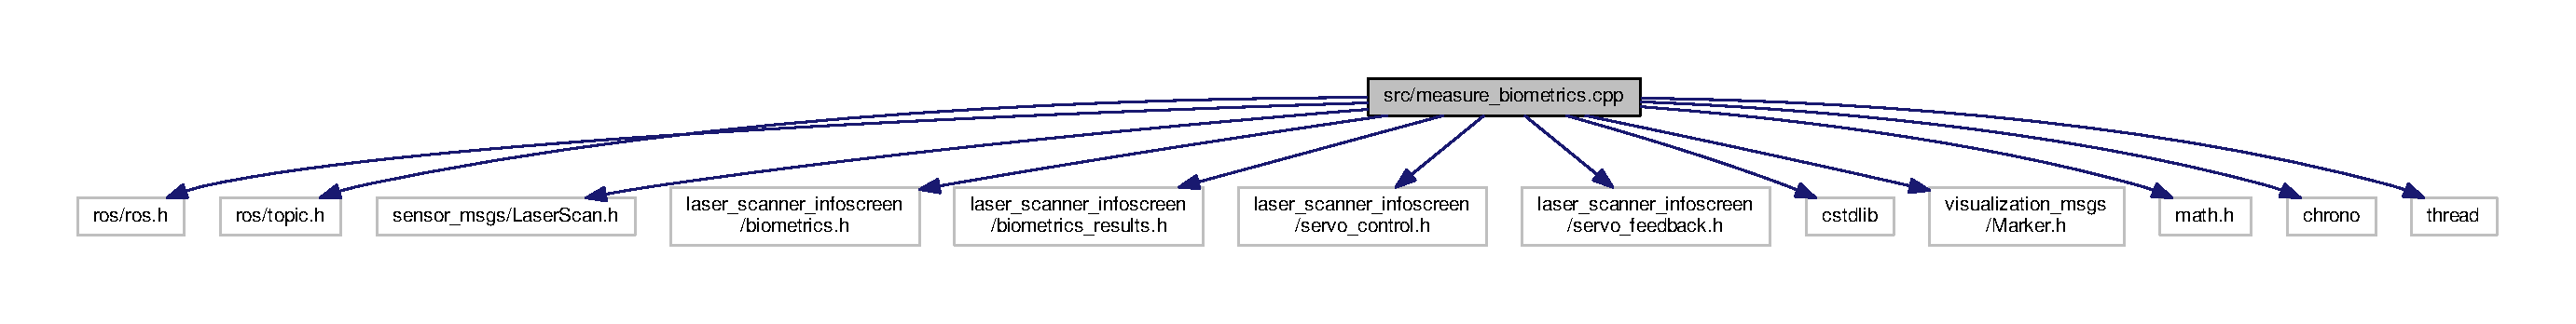
\includegraphics[width=350pt]{measure__biometrics_8cpp__incl}
\end{center}
\end{figure}


\subsection{Detailed Description}
A naive implementation of biometrics measurements. 

A R\+OS Node that uses laserscanner to measure the height of the target. 